\documentclass[11pt]{article}

\usepackage[margin=1in]{geometry}
\usepackage[T1]{fontenc}
\usepackage{lmodern}
\usepackage{microtype}
\DisableLigatures[-]{encoding = T1, family = tt*}
\DeclareTextFontCommand{\texttt}{\normalfont\ttfamily}
\usepackage{amsmath,amssymb,amsthm,mathtools}
\usepackage{array,booktabs,tabularx}
\usepackage{enumitem}
\setlist[enumerate]{beginpenalty=10000}
\usepackage{xcolor}
\usepackage{tikz}
\usetikzlibrary{arrows.meta,positioning,fit,backgrounds,calc}
\usepackage{listings}
\usepackage[colorlinks=true,linkcolor=blue!60!black,citecolor=green!50!black,urlcolor=blue!70!black]{hyperref}

\definecolor{inkblue}{RGB}{24,78,136}
\definecolor{inkteal}{RGB}{15,108,104}
\definecolor{inkgreen}{RGB}{28,112,62}
\definecolor{inkred}{RGB}{165,36,42}
\definecolor{inkamber}{RGB}{168,104,12}
\definecolor{softblue}{RGB}{236,243,252}
\definecolor{softteal}{RGB}{234,246,245}
\definecolor{softgreen}{RGB}{236,248,240}
\definecolor{softred}{RGB}{253,240,240}
\definecolor{softamber}{RGB}{254,247,232}
\definecolor{softgray}{RGB}{244,246,248}

\newcommand{\calloutbox}[3]{%
  \par\medskip\noindent
  \fcolorbox{#1}{#2}{%
    \begin{minipage}{\dimexpr\linewidth-2\fboxsep-2\fboxrule\relax}
      \small #3
    \end{minipage}%
  }\par\medskip
}

\emergencystretch=1.5em
\DeclareRobustCommand{\_}{\ifmmode\sb\else\textunderscore\allowbreak\fi}
\pdfstringdefDisableCommands{%
  \def\BB{BB}%
  \def\_ {\textunderscore}%
  \def\_{\textunderscore}%
}

% Theorem environments
\newtheorem{theorem}{Theorem}[section]
\newtheorem{lemma}[theorem]{Lemma}
\newtheorem{proposition}[theorem]{Proposition}
\newtheorem{corollary}[theorem]{Corollary}
\theoremstyle{definition}
\newtheorem{definition}[theorem]{Definition}
\theoremstyle{remark}
\newtheorem{remark}[theorem]{Remark}
\newtheorem{heuristic}[theorem]{Heuristic Remark (Non-Theorem)}

% Listings configuration for Lean 4 and C snippets
\lstdefinelanguage{Lean4}{
  morekeywords={def,theorem,inductive,structure,where,by,intro,cases,with,if,then,else,let,in,match,unfold,dsimp,only,repeat,split,at,all_goals,first,contradiction,injection,subst,omega,decide,refine,have,rw,simp,calc,macro,namespace,end,import,abbrev,deriving,fun},
  sensitive=true,
  morecomment=[l]{--},
  morecomment=[s]{/-}{-/},
  basicstyle=\ttfamily\footnotesize,
  keywordstyle=\bfseries\color{blue!65!black},
  commentstyle=\itshape\color{gray!75!black},
  columns=fullflexible,
  keepspaces=true,
  frame=single,
  rulecolor=\color{black!25}
}

\lstset{
  basicstyle=\ttfamily\footnotesize,
  columns=fullflexible,
  keepspaces=true,
  frame=single,
  rulecolor=\color{black!25},
  literate={\`}{{\textasciigrave}}1
}

\newcommand{\BB}{\mathrm{BB}}
\newcommand{\Z}{\mathbb{Z}}
\newcommand{\Q}{\mathbb{Q}}
\newcommand{\N}{\mathbb{N}}
\newcommand{\R}{\mathbb{R}}
\newcommand{\Halt}{\mathbf{Halt}}
\newcommand{\rk}{\mathrm{rk}}

\hypersetup{pdftitle={Following a Six-State Busy Beaver Candidate for 97 Quadrillion Steps: Certified Tape Rules, Cross-Library Proofs, and Two Open Endings},pdfauthor={Darryl Novotny},pdfsubject={Exact tape rules, semantic interoperability, and two open questions about the blank run},pdfkeywords={Busy Beaver, Turing machines, Lean, nonhalting}}
\title{\textbf{Following a Six-State Busy Beaver Candidate\\ for 97 Quadrillion Steps}\\ \vspace{0.35em}
\large Certified Tape Rules, Cross-Library Proofs, and Two Open Endings}
\author{Darryl Novotny\\SyncQutrit Research Group, LLC.\\\href{mailto:darryl@syncqutrit.com}{darryl@syncqutrit.com}}
\date{November 18, 2026}
\begin{document}
\maketitle
\begin{abstract}
How far can we follow a machine whose entire rule table has twelve entries? We study AppC~8, a six-state machine in the Busy Beaver search. Its head crosses some stretches of tape in a predictable way. We prove what changes on each crossing and use those rules to follow the machine through more than 97 quadrillion steps from a blank tape. Whether it ever stops remains open. We identify two families of tape endings. Proving a return rule for each family would show that the machine runs forever. A second machine, AppC~7, illustrates what we can learn when the outcome is already known. We count exactly how long it takes to halt from two families of prepared tapes. Together with an existing proof that AppC~7 runs forever from blank, this shows that its blank run can never enter either family. The proofs are available in Lean, a system for checking mathematical arguments.
\end{abstract}

\section{How long can six states keep a machine running?}
\label{sec:scope}
A Turing machine has a head that moves along a tape. At each step it reads the symbol under the head, writes a symbol, moves one square, and changes state according to a table. With six states and two symbols, the table has just twelve entries. A missing instruction tells the machine to halt. For a given number of states, the Busy Beaver question asks for the largest step count among machines that eventually halt when started on an all-zero tape. For five states the answer is $47{,}176{,}870$ \cite{bbchallenge2024bb5}. Moving to six states means asking, among other things, which long-running machines will ever stop.

Consider one of those machines, AppC~8, whose entire twelve-entry rule table fits in Table~\ref{tab:appc8rules}. After five steps from an all-zero tape it has written a short pattern that we can recognize. Later it spends whole stretches of its run scanning repeated blocks. If we know what one sweep does to a block, we can prove what the sweep does to a thousand blocks. That lets us count steps we could never reasonably inspect one at a time.

\begin{table}[htbp]
\centering\small
\begin{tabular}{@{}lcccccc@{}}
\toprule
Read & State $A$ & State $B$ & State $C$ & State $D$ & State $E$ & State $F$ \\
\midrule
\texttt{0} & \texttt{1RB} & \texttt{1LA} & \texttt{0LB} & \texttt{1RE} & \texttt{1LC} & \texttt{0LA} \\
\texttt{1} & \texttt{1LC} & \texttt{0RD} & \texttt{1LF} & \texttt{1LC} & \texttt{0RB} & \textcolor{inkred}{\texttt{---}} \\
\bottomrule
\end{tabular}
\caption{The complete twelve-entry rule table for AppC~8 (\texttt{1RB1LC\_1LA0RD\_0LB1LF\_1RE1LC\_1LC0RB\_0LA---}). Each entry specifies symbol written, head move (\texttt{L}/\texttt{R}), and next state; \texttt{---} at $(F,1)$ halts.}
\label{tab:appc8rules}
\end{table}

\paragraph{A sweep you can count.}
Write $C(k,m)$ for a particular tape configuration. The head is in state $A$ reading a zero. To its right are the symbols $10$, then $k$ copies of $110$, then $m$ ones. All other squares are zero. AppC~8 reaches $C(18,10)$ after 3,244 steps from blank. As Figure~\ref{fig:shuttle} illustrates, a shuttle round across the blocks uses up four of the trailing ones and adds two copies of $110$, taking $12k+26$ steps whenever $m\ge5$. For $C(18,10)$, the first round takes 242 steps and the next takes 266:
\[
 C(18,10)\ \xrightarrow{242}\ C(20,6)\ \xrightarrow{266}\ C(22,2).
\]
Now only two ones remain. The shuttle needs at least five, so we need a different rule. Appendix~\ref{sec:appc8raw} derives the rule from the twelve instructions and gives its cost for any allowed number of blocks.

\begin{figure}[htbp]
\centering
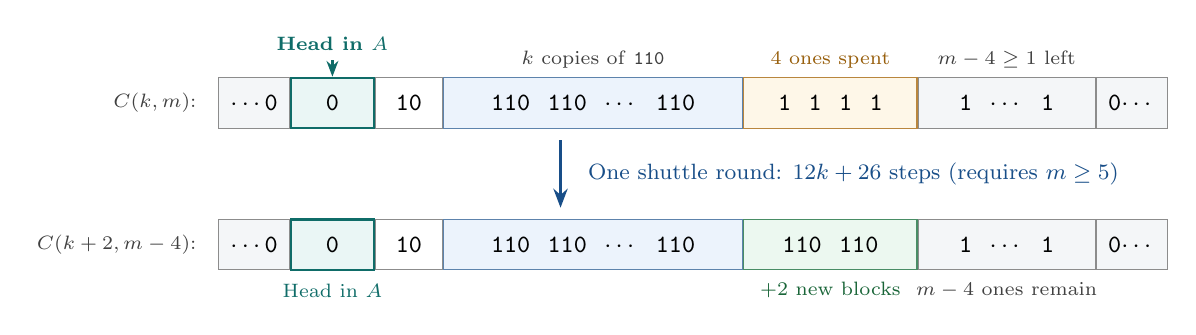
\begin{tikzpicture}[
  cell/.style={draw=black!45, minimum height=0.64cm, inner sep=2pt, font=\ttfamily\small, anchor=west},
  lbl/.style={font=\scriptsize, text=black!75}
]
  % Top tape: C(k,m)
  \node[lbl, anchor=east] at (-0.15, 2.05) {$C(k,m)$:};
  \node[cell, fill=softgray, minimum width=0.9cm] (t0) at (0, 2.05) {$\cdots$0};
  \node[cell, fill=softteal, draw=inkteal, thick, minimum width=1.05cm] (th) at (t0.east) {0};
  \node[cell, fill=white, minimum width=0.85cm] (tp) at (th.east) {10};
  \node[cell, fill=softblue, draw=inkblue!70, minimum width=3.8cm] (tk) at (tp.east) {110\, 110\, $\cdots$\, 110};
  \node[cell, fill=softamber, draw=inkamber!80, minimum width=2.2cm] (t4) at (tk.east) {1\, 1\, 1\, 1};
  \node[cell, fill=softgray, minimum width=2.25cm] (tr) at (t4.east) {1\, $\cdots$\, 1};
  \node[cell, fill=softgray, minimum width=0.9cm] (te) at (tr.east) {0$\cdots$};

  % Head pointer top
  \node[font=\scriptsize\bfseries, text=inkteal] (headtop) at ($(th.north)+(0,0.42)$) {Head in $A$};
  \draw[-{Stealth[length=2mm]}, inkteal, thick] (headtop.south) -- (th.north);

  % Top annotations
  \node[lbl] at ($(tk.north)+(0,0.22)$) {$k$ copies of \texttt{110}};
  \node[lbl, text=inkamber!90!black] at ($(t4.north)+(0,0.22)$) {4 ones spent};
  \node[lbl] at ($(tr.north)+(0,0.22)$) {$m-4\ge1$ left};

  % Transition arrow
  \draw[-{Stealth[length=2.4mm]}, inkblue, very thick] (4.35, 1.58) -- (4.35, 0.72)
    node[midway, right=6pt, font=\footnotesize, text=inkblue] {One shuttle round: $12k+26$ steps (requires $m\ge5$)};

  % Bottom tape: C(k+2, m-4)
  \node[lbl, anchor=east] at (-0.15, 0.25) {$C(k+2,m-4)$:};
  \node[cell, fill=softgray, minimum width=0.9cm] (b0) at (0, 0.25) {$\cdots$0};
  \node[cell, fill=softteal, draw=inkteal, thick, minimum width=1.05cm] (bh) at (b0.east) {0};
  \node[cell, fill=white, minimum width=0.85cm] (bp) at (bh.east) {10};
  \node[cell, fill=softblue, draw=inkblue!70, minimum width=3.8cm] (bk) at (bp.east) {110\, 110\, $\cdots$\, 110};
  \node[cell, fill=softgreen, draw=inkgreen!80, minimum width=2.2cm] (b2) at (bk.east) {110\, 110};
  \node[cell, fill=softgray, minimum width=2.25cm] (br) at (b2.east) {1\, $\cdots$\, 1};
  \node[cell, fill=softgray, minimum width=0.9cm] (be) at (br.east) {0$\cdots$};

  % Bottom annotations
  \node[lbl, text=inkteal] at ($(bh.south)+(0,-0.25)$) {Head in $A$};
  \node[lbl, text=inkgreen!90!black] at ($(b2.south)+(0,-0.25)$) {$+2$ new blocks};
  \node[lbl] at ($(br.south)+(0,-0.25)$) {$m-4$ ones remain};
\end{tikzpicture}
\caption{Anatomy of one certified AppC~8 shuttle round (Theorem~\ref{thm:appc8shuttle}). Four trailing ones are converted into two \texttt{110} blocks while keeping $2k+m$ unchanged at the endpoints; at least one trailing one must survive ($m\ge5$) to turn the head around cleanly.}
\label{fig:shuttle}
\end{figure}

\paragraph{What a long run tells us.}
By joining such rules, we can account for every step from blank up to $97{,}311{,}884{,}181{,}777{,}598$. Lean, a proof assistant, checks that the rules fit together and that each one follows from the machine instructions. This count belongs to one machine whose eventual fate remains open. To use its run to raise the Busy Beaver lower bound, we would also have to show that the machine eventually halts.

\calloutbox{inkblue!45}{softblue}{%
  \textbf{Contributions and evidence scope at a glance.}
  \begin{enumerate}[leftmargin=1.4em,itemsep=2pt,topsep=3pt,parsep=0pt]
    \item \textbf{Certified blank run (AppC~8):} A kernel-checked raw-tape proof follows AppC~8 from blank to step $97{,}311{,}884{,}181{,}777{,}598$ with every earlier step defined, transported into DeepMind's upstream Lean semantics (Appendices~\ref{sec:appc8raw}--\ref{sec:grammarproof}).
    \item \textbf{Suffix grammar and two open predicates (AppC~8):} Universal fuel-burning carry laws close five of six grammar families and three of five paired subcases, reducing blank-tape nonhalting to two explicit open return predicates while proving why an earlier broader family fails via a 749-step halting witness (Section~\ref{sec:grammar}, Appendix~\ref{sec:grammarproof}).
    \item \textbf{Cross-library gate exclusion (AppC~7):} Exact quadratic halting-attempt formulas for two nonblank gate families combine with the upstream blank-tape nonhalting proof via a proved semantic adapter to show neither gate family is reachable from blank (Section~\ref{sec:appc7story}, Appendices~\ref{sec:appc7raw} and~\ref{sec:interop}).
    \item \textbf{Counter models, algebraic certificates, and loop shortcuts:} Model-level aperiodicity, finite A.11 evaluations, conditional Antihydra algebra, a direct raw nonhalting proof for the bipartite bouncer, and guarded \texttt{CLZ}/\texttt{CTZ} benchmarks, with model proofs, raw proofs, and finite tests kept strictly separate (Section~\ref{sec:carryover}, Appendices~\ref{sec:drift}--\ref{sec:reproduce}).
  \end{enumerate}
}

\section{Two patterns still to explain}
\label{sec:grammar}
What would turn a long finite calculation into a proof that the run continues forever? One approach is to find a family of tape configurations that the blank run enters, then show that from \emph{every} member the machine reaches another member after at least one step. Repeating that argument would cover any finite number of steps.

Choosing the family matters. One early candidate admitted a nonblank configuration in which the fixed prefix $10$ is followed by runs of ones of lengths $2,1,5,5,5,2$, separated by zeros. From that configuration the machine completes 748 transitions and encounters an undefined instruction on attempt 749. A family that includes it cannot support the proposed return argument. The example tells us which tapes to exclude even though its starting tape differs from the blank one.

We now describe the ends of the tapes by rules for the lengths of the runs of ones. This \emph{grammar} admits six infinite families of endings and excludes the earlier counterexample. Its behavior is driven by a universal fuel-burning carry law on lone trailing runs of $3r+2$ ones:
\begin{itemize}[leftmargin=1.4em,itemsep=2pt,topsep=3pt]
  \item \textbf{Even carry ($3r+2=6q+2$):} the head burns $q$ left blocks and stretches the ending to $9q+5$ ones. Two consecutive even carries send $44\mapsto104\mapsto239$ along the actual blank run.
  \item \textbf{Odd carry ($3r+2=6q+5$):} the head burns $q+1$ left blocks and \emph{splits} the ending into a paired suffix of $9q+8$ ones, a zero, and two final ones.
  \item \textbf{Short fuel:} if the left tape holds too few blocks for the sweep, the excursion finishes early and collapses cleanly back to a suffix-free tape.
\end{itemize}
Together, these rules prove that every configuration $C_{\,0\,1^{3r+2}}(k,1)$ returns to the grammar for all nonnegative $k$ and $r$, covering both marker patterns used when the head comes back across the tape.

That odd-carry split explains why paired endings always take the form $0\,1^{9q+8}\,0\,1^2$. Five of the six grammar families---and three of the five subcases inside the paired family ($m=2$, $m=4$, and $m\ge5$)---are already proved to return unconditionally (Figure~\ref{fig:grammar}). Only two cases would finish this particular argument. In both, the tape ends with $t=0\,1^{9q+8}\,0\,1^2$, preceded by a run of either one or three ones:
\[
 C_t(k,1)\quad\text{and}\quad C_t(k,3),\qquad
 t=0\,1^{9q+8}\,0\,1^2 .
\]
For each choice, the question is the same: for every block count $k\ge0$ and every $q\ge0$, does the machine reach a configuration in the grammar again after a positive number of steps? The latest certified point on the blank run has the second form, with $k=134{,}241{,}197$ and $q=39$ (last two runs of lengths 359 and 2). All 2,050 paired inputs in a bounded search returned to the grammar, but a proof for arbitrary $k$ and $q$ is still missing for both forms. Appendix~\ref{sec:grammarproof} gives the exact grammar, universal carry laws, and search limits.

\begin{figure}[htbp]
\centering
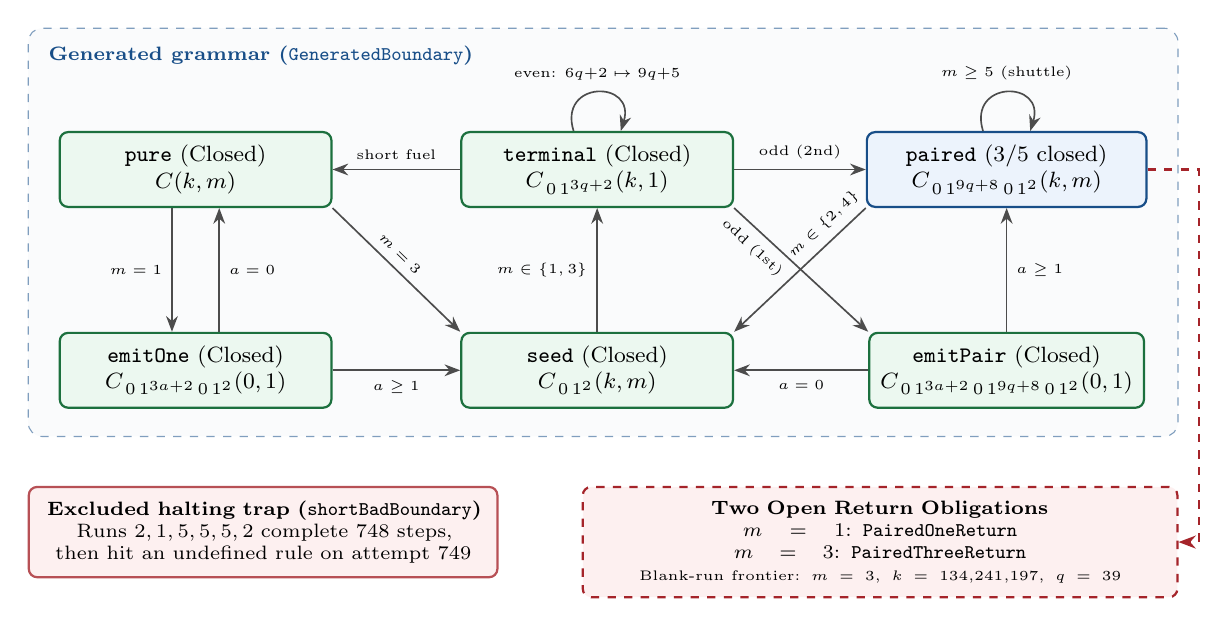
\begin{tikzpicture}[
  gnode/.style={draw=inkgreen, fill=softgreen, rounded corners=3pt, thick, align=center, font=\footnotesize, minimum width=3.45cm, minimum height=0.95cm, inner sep=4pt},
  pnode/.style={draw=inkblue, fill=softblue, rounded corners=3pt, thick, align=center, font=\footnotesize, minimum width=3.55cm, minimum height=0.95cm, inner sep=4pt},
  onode/.style={draw=inkred, fill=softred, dashed, rounded corners=3pt, thick, align=center, font=\scriptsize, text width=7.2cm, inner sep=5pt},
  tnode/.style={draw=inkred!80, fill=softred, rounded corners=3pt, thick, align=center, font=\scriptsize, text width=5.6cm, inner sep=5pt},
  arr/.style={-{Stealth[length=2mm]}, semithick, draw=black!70},
  oarr/.style={-{Stealth[length=2.2mm]}, thick, dashed, draw=inkred}
]
  % Six GeneratedCode nodes in a clean 3x2 grid
  \node[gnode] (pure) at (0, 2.55) {\textbf{\texttt{pure}} (Closed)\\$C(k,m)$};
  \node[gnode] (term) at (5.1, 2.55) {\textbf{\texttt{terminal}} (Closed)\\$C_{\,0\,1^{3q+2}}(k,1)$};
  \node[pnode] (paired) at (10.3, 2.55) {\textbf{\texttt{paired}} (3/5 closed)\\$C_{\,0\,1^{9q+8}\,0\,1^2}(k,m)$};

  \node[gnode] (e1) at (0, 0.0) {\textbf{\texttt{emitOne}} (Closed)\\$C_{\,0\,1^{3a+2}\,0\,1^2}(0,1)$};
  \node[gnode] (seed) at (5.1, 0.0) {\textbf{\texttt{seed}} (Closed)\\$C_{\,0\,1^2}(k,m)$};
  \node[gnode] (ep) at (10.3, 0.0) {\textbf{\texttt{emitPair}} (Closed)\\$C_{\,0\,1^{3a+2}\,0\,1^{9q+8}\,0\,1^2}(0,1)$};

  % Self-loops cleanly above top row (with named label nodes included in fit)
  \draw[arr] ([xshift=-3mm]term.north) .. controls +(-0.2,0.65) and +(0.2,0.65) .. ([xshift=3mm]term.north)
    node[midway, above=1pt, font=\tiny] (termloop) {even: $6q{+}2\mapsto9q{+}5$};
  \draw[arr] ([xshift=-3mm]paired.north) .. controls +(-0.2,0.65) and +(0.2,0.65) .. ([xshift=3mm]paired.north)
    node[midway, above=1pt, font=\tiny] (pairloop) {$m\ge5$ (shuttle)};

  % Proved internal transitions (non-overlapping labels)
  \draw[arr] ([xshift=-3mm]pure.south) -- ([xshift=-3mm]e1.north) node[midway, left, font=\tiny] {$m=1$};
  \draw[arr] ([xshift=3mm]e1.north) -- ([xshift=3mm]pure.south) node[midway, right, font=\tiny] {$a=0$};
  \draw[arr] (e1.east) -- (seed.west) node[midway, below, font=\tiny] {$a\ge1$};
  \draw[arr] (pure.south east) -- (seed.north west) node[pos=0.45, sloped, above, font=\tiny] {$m=3$};
  \draw[arr] (seed.north) -- (term.south) node[midway, left, font=\tiny] {$m\in\{1,3\}$};
  \draw[arr] (term.west) -- (pure.east) node[midway, above, font=\tiny] {short fuel};
  \draw[arr] (term.east) -- (paired.west) node[midway, above, font=\tiny] {odd (2nd)};
  \draw[arr] (term.south east) -- (ep.north west) node[pos=0.22, sloped, below, font=\tiny] {odd (1st)};
  \draw[arr] (ep.north) -- (paired.south) node[midway, right, font=\tiny] {$a\ge1$};
  \draw[arr] (ep.west) -- (seed.east) node[midway, below, font=\tiny] {$a=0$};
  \draw[arr] (paired.south west) -- (seed.north east) node[pos=0.23, sloped, above, font=\tiny] {$m\in\{2,4\}$};

  % Dashed frame cleanly enclosing all six nodes AND self-loop labels
  \begin{scope}[on background layer]
    \node[draw=inkblue!55, dashed, rounded corners=5pt, fill=softgray!45,
          fit=(pure)(term)(paired)(e1)(seed)(ep)(termloop)(pairloop), inner xsep=11pt, inner ysep=10pt] (frame) {};
    \node[font=\scriptsize\bfseries, text=inkblue, anchor=north west] at ($(frame.north west)+(4pt,-3pt)$) {Generated grammar (\texttt{GeneratedBoundary})};
  \end{scope}

  % Excluded halting trap (bottom left, cleanly separated)
  \node[tnode, anchor=north west] (trap) at ($(frame.south west)+(0,-0.62)$) {%
    \textbf{Excluded halting trap (\texttt{shortBadBoundary})}\\
    Runs $2,1,5,5,5,2$ complete 748 steps,\\
    then hit an undefined rule on attempt 749
  };

  % Open obligations (bottom right, cleanly separated)
  \node[onode, anchor=north east] (open) at ($(frame.south east)+(0,-0.62)$) {%
    \textbf{Two Open Return Obligations}\\
    $m=1$: \texttt{PairedOneReturn}\\
    $m=3$: \texttt{PairedThreeReturn}\\
    {\tiny Blank-run frontier: $m=3,\ k=134{,}241{,}197,\ q=39$}
  };

  \draw[oarr] (paired.east) -- ++(0.65,0) |- (open.east);
\end{tikzpicture}
\caption{Transition structure of the six \texttt{GeneratedCode} suffix families. Solid arrows denote universally proved Lean return laws (including intermediate fuel-drain and shuttle phases). Only the two dashed red exits from \texttt{paired} remain open; the earlier 749-step halting counterexample lies strictly outside the grammar.}
\label{fig:grammar}
\end{figure}

\calloutbox{inkred!55}{softred}{%
  \textbf{Open Challenge: Closing AppC~8.}
  Let $t=0\,1^{9q+8}\,0\,1^2$. Proving either predicate below settles half of the remaining conditional closure theorem \texttt{generated\_closure\_of\_paired}; proving both immediately yields an unconditional proof of \texttt{BusyBeaver.IsNotHalt} via \texttt{upstream\_nonhalting\_of\_paired}:
  \begin{itemize}[leftmargin=1.4em,itemsep=1pt,topsep=2pt,parsep=0pt]
    \item \texttt{PairedOneReturn}: for all $k,q\in\N$, $C_t(k,1)$ reaches \texttt{GeneratedBoundary} in positive time.
    \item \texttt{PairedThreeReturn}: for all $k,q\in\N$, $C_t(k,3)$ reaches \texttt{GeneratedBoundary} in positive time (current certified blank-run frontier: $k=134{,}241{,}197,\ q=39$).
  \end{itemize}
  Conversely, finding a single halting or non-returning $(k,q)$ witness refutes that premise and pinpoints how the grammar must be narrowed, just as \texttt{shortBadBoundary} did earlier.
}

\section{What a different starting tape can teach us}
\label{sec:appc7story}
A second machine, AppC~7, illustrates a different use for an exact step count. The proof library from Google DeepMind and the cryptids contributors already establishes that this machine runs forever from a blank tape \cite{deepmind2026cryptidsSnapshot}. We asked which combinations of tape, head position, and state could occur during that run.

Start it instead on one of two specified families of nonblank tapes. We call each such configuration a \emph{gate} because entering it commits the machine to a particular outcome. We prove that every gate in either family leads to a halt. For the smallest member of the prefixed family, the machine completes 14 steps and finds its next instruction undefined on attempt 15. Appendix~\ref{sec:appc7raw} gives the exact count as the pattern grows.

If the machine ever reached a gate from blank, it would follow the same instructions from there and halt. That would contradict the existing proof for the blank tape. To combine the two results across independent codebases and Lean versions, we built a semantic adapter $\Phi$ proving that our tape zipper and the upstream quotient tape agree after every instruction, including undefined ones (Figure~\ref{fig:interop}, Appendix~\ref{sec:interop}).

\begin{figure}[htbp]
\centering
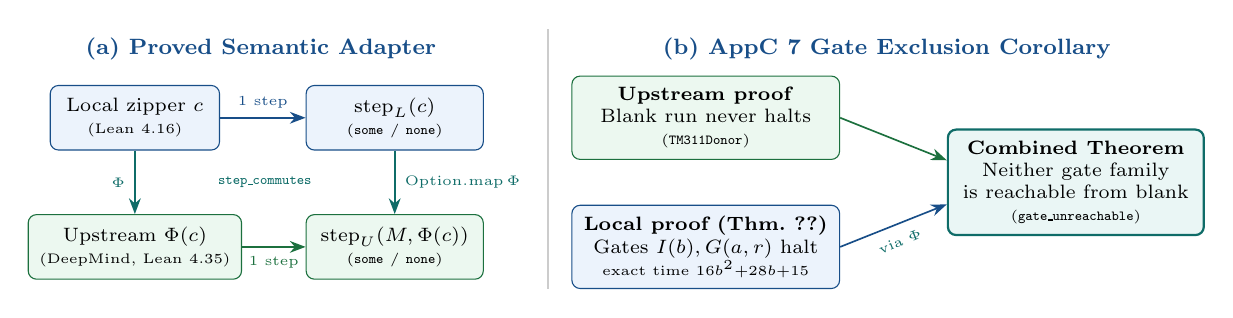
\begin{tikzpicture}[
  box/.style={draw=black!55, rounded corners=3pt, align=center, font=\scriptsize, inner sep=4pt, minimum height=0.82cm},
  arr/.style={-{Stealth[length=2mm]}, semithick}
]
  % Left panel: Commuting square
  \node[font=\footnotesize\bfseries, text=inkblue] at (2.4, 2.8) {(a) Proved Semantic Adapter};
  \node[box, fill=softblue, draw=inkblue, minimum width=2.15cm] (lc) at (0.8, 1.92) {Local zipper $c$\\ {\tiny (Lean 4.16)}};
  \node[box, fill=softblue, draw=inkblue, minimum width=2.25cm] (ln) at (4.1, 1.92) {$\operatorname{step}_L(c)$\\ {\tiny (\texttt{some} / \texttt{none})}};
  \node[box, fill=softgreen, draw=inkgreen, minimum width=2.15cm] (uc) at (0.8, 0.28) {Upstream $\Phi(c)$\\ {\tiny (DeepMind, Lean 4.35)}};
  \node[box, fill=softgreen, draw=inkgreen, minimum width=2.25cm] (un) at (4.1, 0.28) {$\operatorname{step}_U(M,\Phi(c))$\\ {\tiny (\texttt{some} / \texttt{none})}};

  \draw[arr, inkblue] (lc) -- (ln) node[midway, above, font=\tiny] {1 step};
  \draw[arr, inkgreen] (uc) -- (un) node[midway, below, font=\tiny] {1 step};
  \draw[arr, inkteal] (lc) -- (uc) node[midway, left, font=\tiny] {$\Phi$};
  \draw[arr, inkteal] (ln) -- (un) node[midway, right, font=\tiny] {$\mathrm{Option.map}\,\Phi$};
  \node[font=\tiny\bfseries, text=inkteal] at (2.45, 1.1) {\texttt{step\_commutes}};

  % Divider
  \draw[black!20, thick] (6.05, -0.25) -- (6.05, 3.05);

  % Right panel: Gate exclusion deduction
  \node[font=\footnotesize\bfseries, text=inkblue] at (10.35, 2.8) {(b) AppC~7 Gate Exclusion Corollary};
  \node[box, fill=softgreen, draw=inkgreen, minimum width=3.4cm] (up) at (8.05, 1.92) {\textbf{Upstream proof}\\Blank run never halts\\ {\tiny (\texttt{TM311Donor})}};
  \node[box, fill=softblue, draw=inkblue, minimum width=3.4cm] (loc) at (8.05, 0.28) {\textbf{Local proof (Thm.~\ref{thm:appc7gate})}\\Gates $I(b), G(a,r)$ halt\\ {\tiny exact time $16b^2{+}28b{+}15$}};
  \node[box, fill=softteal, draw=inkteal, thick, minimum width=3.25cm, minimum height=1.28cm] (res) at (12.75, 1.1) {\textbf{Combined Theorem}\\Neither gate family\\is reachable from blank\\ {\tiny (\texttt{gate\_unreachable})}};

  \draw[arr, inkgreen] (up.east) -- ($(res.west)+(0,0.28)$);
  \draw[arr, inkblue] (loc.east) -- ($(res.west)+(0,-0.28)$) node[midway, sloped, below=1pt, font=\tiny, text=inkteal] {via $\Phi$};
\end{tikzpicture}
\caption{Cross-library verification architecture. (a)~The adapter $\Phi$ commutes with single-step and multi-step execution, including halting transitions. (b)~Transporting our exact local halting witnesses into DeepMind's upstream nonhalting theorem proves that neither AppC~7 gate family can ever appear on the blank run.}
\label{fig:interop}
\end{figure}

\section{What carries over to other machines?}
\label{sec:carryover}
A repeated tape pattern often suggests keeping just a few numbers, such as the lengths of two blocks. In several of our resulting counter models we can find a quantity that grows at every step the model takes. Returning to an earlier state would give the quantity its old value, which is impossible. The model can still reach a state with no next step. To apply the result to a particular machine one must also prove that its instructions implement the counter rules on the tapes in question.

The distinction shows up in BMO~8. Here the sum of two counters grows by either three or five on each defined step within the specified domain. We can also describe exactly which counter pairs halt at the next step. They fall into three families. The growth calculation alone leaves open whether the starting counters will ever reach one of them (Appendix~\ref{sec:core}). In another example, the bipartite bouncer, the instructions themselves keep every odd-numbered tape cell at zero on the blank run. That restriction keeps the machine away from its halting instruction (Appendix~\ref{sec:bouncer}).

These examples build on Rad\'o's question \cite{rado1962noncomputable}, early computational studies \cite{lin1965computer,brady1983determination,marxen1990attacking}, and Michel's analysis of the arithmetic behind small machines \cite{michel2015busy}. We use the machine labels of Dos Santos et al.\ \cite{dossantos2026limits}. Their term \emph{cryptid} describes a machine with compact rules whose blank-tape halting behavior remains unresolved. Their A.1--A.11 machines already have formally checked accelerations. Connecting each of our counter models to those tape-level rules remains a separate task. Table~\ref{tab:domains} in Appendix~\ref{sec:core} lists the precise domains.

For readers who would like to contribute, the two paired endings in Section~\ref{sec:grammar} offer a specific place to start. A return rule that works for either entire family would settle one premise. A single member that never returns would rule out that premise and help explain which tapes a revised family should include. An earlier counterexample led us to the grammar we use today.

\clearpage
\appendix
\section{From individual instructions to exact tape rules}
The appendices give the machine tables, the hypotheses of each rule, and the Lean names used to check them. Throughout, $\N$ includes zero. In a tape word, $1^m$ means $m$ consecutive ones, and $(110)^k$ means $k$ consecutive copies of the three-symbol block. A configuration includes the tape, the position of the head relative to the displayed word, and the control state; we write $\langle Q:b\rangle$ for the head in control state $Q$ scanning symbol $b$. An arrow labelled by $n$ means that the machine completes $n$ instructions between the displayed endpoints.

\subsection{How long AppC 7 takes to halt from a gate}
We use the AppC~7 machine identified by its full table in the pinned repository \cite{deepmind2026cryptidsSnapshot}. Our initial tapes are nonblank. Appendix~\ref{sec:interop} uses the upstream blank-tape result to exclude the gates from that run.

\label{sec:appc7raw}
The module \texttt{AppC7RawGate.lean} defines the following machine. Each group contains the two instructions for one state, in reading order 0 then 1. For example, $1RB$ means write 1, move right, and enter state $B$. Three dashes mark an undefined instruction.
\begin{center}\small\texttt{1RB1RC\_1LC0LE\_0RA1RD\_1RF1LB\_1LD0LA\_---0RC}
\end{center}
The raw configuration is a finite tape zipper: the left list stores cells nearest the head first, the right list starts with the scanned cell, and every missing cell is zero. One step performs exactly the table's write, left/right move, and state change, or returns no successor at $F0$. There are no counter-level or macro rules in this step function.

\begin{theorem}[Exact AppC 7 gate family]
\label{thm:appc7gate}
For every $a,r\in\N$, start in state $D$ on the zero immediately left of $(10)^a(1110)^r11$, with all other unlisted cells zero. The first undefined instruction is attempted at
\[
T(a,r)=16r^2+(8a+12)r+2a+5.
\]
Equivalently, the machine executes exactly $T(a,r)-1$ defined transitions and is then in state $F$ scanning zero. Starting instead at $\langle A:0\rangle\,00(1110)^b11$, the first halting attempt is $16b^2+28b+15$ for every $b\in\N$. Every shorter execution prefix is defined.
\end{theorem}
\begin{proof}
The raw sweep theorem \texttt{gate\_phase\_all} proves, for every $a$ and arbitrary finite right tail, that one $1110$ block is consumed and the $10$ prefix grows by four in $8a+20$ defined steps. For $a\ge1$, the proof composes three entry instructions, a $2(a-1)$-step right scan, ten turn instructions, a $6(a-1)$-step return scan, and fifteen boundary instructions; the zero-prefix case is checked directly in twenty instructions. With no $1110$ blocks remaining, \texttt{gate\_terminal\_all} reaches $F0$ in $2a+4$ defined transitions. Induction on $r$ therefore refines the recurrence
\[
T(a,0)=2a+5,\qquad T(a,r+1)=8a+20+T(a+4,r).
\]
The existing arithmetic closed form then gives the displayed polynomial. A six-instruction prefix maps the $A$-state family into the $D$-state family with $a=2$. The theorems \texttt{gate\_sweep\_exact\_time} and \texttt{appC7\_raw\_gate\_exact\_time} prove that all earlier prefixes remain defined, so these are first halting times rather than upper bounds.
\end{proof}
The simulator counts the final attempt, so its halting count is one greater than the number of completed transitions. The unrestricted multi-defect word system in Appendix~\ref{sec:transfers} is a separate model.

Independent regression checks compare all twelve table entries with the existing dictionary-tape simulator, test 117 general gate inputs, 33 prefixed inputs, and 403 one-phase inputs with varying right tails. An additional 192 concrete execution comparisons are generated by that simulator and checked in Lean. These finite tests check transcription and execution conventions; the universally quantified result is the inductive Lean proof.

\subsection{How one AppC 8 shuttle round changes the tape}
\label{sec:appc8raw}
The module \texttt{AppC8RawShuttle.lean} defines the complete raw table
\begin{center}\small\texttt{1RB1LC\_1LA0RD\_0LB1LF\_1RE1LC\_1LC0RB\_0LA---}
\end{center}
and explicit read, write, movement, and partial iteration on a head-relative tape zipper. Missing cells are zero. Let $C(k,m)$ denote state $A$ scanning the zero immediately left of $10(110)^k1^m$, with zero-filled unlisted cells.

\begin{theorem}[Raw AppC 8 shuttle and repeated rounds]
\label{thm:appc8shuttle}
For every $k\in\N$ and $m\ge5$, the raw machine reaches $C(k+2,m-4)$ from $C(k,m)$ after $12k+26$ defined transitions. Every prefix through that time is defined. More generally, if $r\in\N$ and $m\ge4r+1$, it reaches $C(k+2r,m-4r)$ after
\[
S(k,r)=12rk+12r(r-1)+26r
\]
defined transitions.
\end{theorem}
\begin{proof}
The theorem \texttt{shuttle\_with\_tail} proves the stronger local statement with an arbitrary finite suffix after the first five trailing ones; the suffix remains unchanged. It composes three entry instructions, a $3k$-step right scan, a five-instruction turn, a $3k$-step left scan, four boundary instructions, a $3(k+1)$-step right scan, a second five-instruction turn, a $3(k+1)$-step left scan, and three final boundary instructions. Their sum is $12k+26$. Each right-scan triplet uses the literal $E,B,D$ instructions to rewrite $110$ as $001$; the return scan and boundary lemmas certify the full resulting tape, including the cases $k=0$ and $m=5$. No macro rule is assumed by the raw step function.

Specializing the unchanged suffix gives \texttt{appC8\_raw\_shuttle}. Successful partial iteration implies that every earlier prefix is defined, formalized by \texttt{appC8\_shuttle\_survives}. Induction on $r$, with the guard $m\ge4r+1$ ensuring at least five ones before each round, gives \texttt{appC8\_raw\_shuttle\_rounds}. Applying the existing closed form for the sum of round durations yields \texttt{appC8\_raw\_rounds\_closed\_form} and $S(k,r)$.
\end{proof}
The duration gives a time at which the displayed configuration occurs. It need not be the first such time. At the two endpoints, \texttt{appC8\_shuttle\_conserves\_2k\_plus\_m} gives the same value of $2k+m$, although the displayed word grows by two cells. The identity concerns the endpoints of the round.

Substituting $k=3$, $m=12q+10$, and $r=3q+2$ gives the raw middle-stage theorem \texttt{appC8\_clean\_middle\_raw}, for every $q\in\N$:
\[
C(3,12q+10)\ \xrightarrow{\ S(3,3q+2)\ }\ C(6q+7,2).
\]
Independent tests compare all twelve table entries, 420 single-round cases, 819 cases with varying right tails, 504 repeated-round cases, and 13 clean-middle cases against the dictionary-tape simulator. A further 192 independently generated execution comparisons are checked in Lean. These tests validate transcription and conventions; the universal claims rest on the inductive proof.

\paragraph{Joining the reset, shuttle, and exit.}
A second useful pattern has the head in state $E$. Write $D(c)$ for $10(100)^c1\langle E:0\rangle$, with every unlisted cell zero. The left zipper stores the word in reverse order, as $(100)^c101$ (since $1(001)^c01=(100)^c101$). We call $D(c)$ a clean input when $c$ is a positive multiple of four. The module \texttt{AppC8RawCleanMacro.lean} proves an exact rule for these inputs.

\begin{theorem}[Raw AppC 8 clean macro]
\label{thm:appc8clean}
For every $c\ge1$ and $k\in\N$, the raw reset and exit are
\[
D(c)\xrightarrow{\ 5c+43\ }C(3,3c-2),\qquad
C(k,2)\xrightarrow{\ 3k+6\ }D(k+1).
\]
Consequently, for every $q\in\N$,
\[
D(4(q+1))\xrightarrow{\ 108q^2+332q+238\ }D(6q+8).
\]
Every prefix through the displayed full-macro duration is defined. These are elapsed execution counts; no first-return minimality is asserted.
\end{theorem}
\begin{proof}
For $c=n+1$, five literal entry instructions reach state $A$ with left zipper $(100)^n101$ and four right-hand ones. The inductive lemma \texttt{reset\_scan} consumes each remaining left $100$ block in five instructions and adds three ones on the right. A fixed 43-instruction boundary sequence transforms the resulting configuration into $C(3,3n+1)$. This proves \texttt{appC8\_raw\_reset}, including $c=1$. The boundary lemma preserves an arbitrary suffix after four leading ones.

For the exit, three entry instructions, the previously proved $3k$-step right scan, and three final instructions give \texttt{appC8\_raw\_exit}, including $k=0$. Specializing to $c=4(q+1)$ and $k=6q+7$ gives durations $20q+63$ and $18q+27$. Composing these with the raw middle stage yields \texttt{appC8\_clean\_macro\_raw}. The arithmetic declaration \texttt{appC8\_clean\_macro\_law} supplies the exact sum
\[
(20q+63)+S(3,3q+2)+(18q+27)=108q^2+332q+238.
\]
Successful partial iteration supplies all defined prefixes via \texttt{appC8\_clean\_macro\_survives}.
\end{proof}
The combined theorem \texttt{appC8\_clean\_macro\_raw\_and\_ghost} connects this raw transition to $2(c'+4)=3(c+4)$ for $c=4(q+1)$ and $c'=6q+8$. Independent dictionary-tape checks cover 128 resets ($1\le c\le128$), 129 exits ($0\le k\le128$), and 33 full clean macros ($0\le q\le32$), comparing the complete tape, state, absolute head position, and elapsed duration. A further 33 complete resulting configurations generated independently are checked by Lean's kernel.

Even a clean input can leave this family. Starting with $c=12$, the rule gives $20$, then $32$, then $50$. At 50 a different rule is needed. Appendix~\ref{sec:appc8mod2} shows where a clean input occurs on the blank run.

\subsection{The first checkpoints from blank}
\label{sec:appc8blank}
The module \texttt{AppC8RawBlankReachability.lean} starts in state $A$ with both zipper lists empty, representing the all-zero tape. Table~\ref{tab:appc8blank} records exact head-relative configurations reached from this one initial state. Times count completed defined transitions; they are not first-visit claims.

\begin{table}[htbp]
\centering\small
\begin{tabular}{rll}
\toprule
Elapsed transitions & Reached configuration & Proof component \\
\midrule
5 & $C(0,2)$ & Five literal instructions \\
11 & $D(1)$ & General exit at $k=0$ \\
59 & $C(3,1)$ & General reset at $c=1$ \\
3,244 & $C(18,10)$ & Concrete 3,185-instruction bridge \\
3,752 & $C(22,2)$ & Two general shuttle rounds \\
3,824 & $D(23)$ & General exit at $k=22$ \\
3,982 & $C(3,67)$ & General reset at $c=23$ \\
7,854 & $C(35,3)$ & Sixteen general shuttle rounds \\
\bottomrule
\end{tabular}
\caption{Kernel-certified checkpoints on the AppC 8 blank trajectory. $C$ and $D$ are the configurations defined in Appendix~\ref{sec:appc8raw}.}
\label{tab:appc8blank}
\end{table}

\begin{theorem}[AppC 8 blank reachability and bounded survival]
Starting from the all-zero tape in state $A$, AppC 8 reaches $C(18,10)$ after 3,244 transitions, $D(23)$ after 3,824 transitions, and $C(35,3)$ after 7,854 transitions. Every execution prefix of length $j\le7{,}854$ is defined.
\end{theorem}
\begin{proof}
Five literal instructions give \texttt{appC8\_blank\_entry}. The proved general exit and reset give $D(1)$ and then $C(3,1)$. The declaration \texttt{appC8\_first\_excursion} uses kernel reduction via \texttt{decide} to verify the concrete equality
\[
\operatorname{run}(3185,C(3,1))=\operatorname{some}(C(18,10)).
\]
This finite certificate is not a generalized rule for arbitrary odd inputs. Composing it with the 59-step prefix gives \texttt{appC8\_blank\_shuttle\_entry}. Two proved shuttle rounds take $242+266=508$ transitions; the exit adds 72, giving \texttt{appC8\_blank\_carry\_twenty\_three}. The reset adds 158; sixteen shuttle rounds add $S(3,16)=3{,}872$, yielding \texttt{appC8\_blank\_odd\_frontier}. The prefix theorem \texttt{appC8\_blank\_prefix\_defined} follows from successful partial iteration.
\end{proof}
The finite bridge is part of the kernel-checked proof, with no custom execution axiom or native evaluation oracle. An independent dictionary-tape simulator checks ten full configurations, including the initial state and the intermediate checkpoint $C(20,6)$ at time 3,486. All ten complete outputs are also checked in Lean by direct executions from blank, independently of the compositional route. Absolute head coordinates are tested by the simulator; the Lean configuration statements are head-relative.

\paragraph{Which checkpoints admit the clean rule?}
The carry counts 1 and 23 in Table~\ref{tab:appc8blank} both fall outside the guard $c=4(q+1)$, as \texttt{appC8\_blank\_carry\_guards} confirms. If the run reaches $D(4(q+1))$ at time $n$, then \texttt{appC8\_blank\_clean\_macro\_transfer} gives $D(6q+8)$ at time $n+108q^2+332q+238$. Appendix~\ref{sec:appc8mod2} applies this rule at $q=173$. First we need to follow the run out of $C(35,3)$.

\subsection{Following a tape with three trailing ones}
\label{sec:appc8odd}
The module \texttt{AppC8RawOddSector.lean} extends the raw proof beyond $C(35,3)$. For a finite suffix $t$, write $C_t(k,m)$ for $\langle A:0\rangle10(110)^k1^m t$, with unlisted cells zero. The family proved here has $k\equiv3\pmod4$ and three trailing ones.

\begin{theorem}[Raw odd-sector excursion]
For every $a\in\N$,
\[
C(4a+3,3)\xrightarrow{\ 108a^2+398a+356\ }C(0,18a+31).
\]
Every prefix through this elapsed duration is defined. Consequently the blank trajectory reaches $C(0,175)$ at time 18,306 and $C(86,3)$ at time 41,096, with every prefix through time 41,096 defined.
\end{theorem}
\begin{proof}
The first collapse and terminal collapse are raw execution theorems for every $k\in\N$:
\[
\begin{aligned}
 C(k,3)&\xrightarrow{\ 14k+36\ }C_{011}(0,3k+7),\\
 C_{011}(k,4)&\xrightarrow{\ 14k+44\ }C(0,3k+13).
\end{aligned}
\]
For the first collapse, the previously proved scans give a $(6k+12)$-instruction half-shuttle and a $3(k+1)$-instruction right scan. Eight literal turn instructions, the general $5(k+1)$-instruction reset scan, and eight left-boundary instructions finish the transformation. The terminal collapse uses the same scans with a 16-instruction turn. These prove \texttt{appC8\_odd\_collapse} and \texttt{appC8\_odd\_terminal}, including $k=0$, directly from the raw table.

Induction extends the suffix-preserving shuttle to \texttt{tail\_shuttle\_rounds}. For $k=4a+3$, the first collapse leaves $12a+16$ ones and suffix $011$. Exactly $3a+3$ certified shuttle rounds reach $C_{011}(6a+6,4)$; the terminal collapse then gives $C(0,18a+31)$. The elapsed sum is
\[
(56a+78)+S(0,3a+3)+(84a+128)=108a^2+398a+356.
\]
The resulting theorem is \texttt{appC8\_odd\_excursion\_closed}. Its prefix corollary is \texttt{appC8\_odd\_excursion\_survives}. Taking $a=8$ gives 10,452 transitions from $C(35,3)$ to $C(0,175)$. Composing with the proved blank prefix gives time $7{,}854+10{,}452=18{,}306$. A further 43 shuttle rounds take $S(0,43)=22{,}790$ transitions, yielding $C(86,3)$ at time 41,096. These are \texttt{appC8\_blank\_after\_odd\_excursion}, \texttt{appC8\_blank\_next\_odd\_frontier}, and \texttt{appC8\_blank\_prefix\_41096}.
\end{proof}
The return value $18a+31$ is odd. At every admissible subsequent shuttle endpoint it remains odd, since a round subtracts four. The theorem \texttt{odd\_output\_not\_exit} therefore excludes a trailing count of two at those endpoints, so the established two-ones exit theorem cannot finish this phase. The concrete new endpoint $C(86,3)$ has state $A$, whereas the full clean macro starts at $D(4(q+1))$ in state $E$; \texttt{odd\_frontier\_not\_clean} formalizes their inequality.

The block count 86 leaves remainder two on division by four, so the $4a+3$ rule ends here. The next proof follows that branch into the clean sector. The checkpoints give elapsed times and leave intermediate visits unrestricted.

Independent checks compare 65 first collapses ($0\le k\le64$), 65 terminal collapses over the same range, 33 full excursions ($0\le a\le32$), and 900 suffix-preserving repeated-shuttle inputs. Complete blank configurations are also checked at times 18,306 and 41,096, including absolute head positions. Twenty-two complete resulting configurations from the independent simulator are checked by direct raw executions in Lean. These finite cross-checks complement the universal inductive proof.

\subsection{How the blank run reaches a clean input}
\label{sec:appc8mod2}
The module \texttt{AppC8RawMod2Sector.lean} distinguishes a uniform reduction for all $k\equiv2\pmod4$ from the more specific complete excursion needed at $k=86$. Define the finite suffixes $T_8=01^8 011$ and $T_{26}=01^{26}011$.

\begin{theorem}[Modulo-four reduction and the $16b+6$ branch]
For every $a\in\N$,
\[
 C(4a+2,3)\xrightarrow{\ 108a^2+398a+388\ }C_{T_8}(0,18a+19).
\]
This reduction retains its displayed suffix; it is not a complete suffix-free excursion formula for the entire residue class. For every $b\in\N$, the more specific branch is
\[
\begin{aligned}
 C(16b+6,3)&\xrightarrow{\ 14364b^2+18494b+6438\ }C(54b+36,2),\\
 C(16b+6,3)&\xrightarrow{\ 14364b^2+18656b+6552\ }D(54b+37).
\end{aligned}
\]
Every prefix through the latter duration is defined. The carry $54b+37$ is odd, so this immediate output is not a full clean-macro input.
\end{theorem}
\begin{proof}
Two additional raw collapse lemmas certify
\[
\begin{aligned}
 C_{011}(k,1)&\xrightarrow{\ 14k+90\ }C_{T_8}(0,3k+1) &&(k\ge2),\\
 C_{T_8}(k,1)&\xrightarrow{\ 14k+416\ }C_{T_{26}}(0,3k-8) &&(k\ge5).
\end{aligned}
\]
These are \texttt{defect\_one\_collapse} and \texttt{defect\_eight\_collapse}. They compose the inductively proved right, return, and reset scans with fixed local instruction sequences. The first collapse uses 19- and 66-instruction turns; the second uses 104- and 334-instruction turns. Each fixed sequence reduces directly in the kernel, with the unvisited left tail parameterized. No macro correspondence is assumed.

Apply the earlier odd collapse at $k=4a+2$, then $3a+3$ suffix-preserving shuttle rounds, then the first new collapse. This gives \texttt{appC8\_mod2\_reduction\_closed}. For $a=4b+1$, the resulting $72b+37$ ones permit $18b+9$ rounds, leaving $C_{T_8}(36b+18,1)$. The second collapse gives $C_{T_{26}}(0,108b+46)$. Another $27b+11$ rounds leave two ones before the zero in $T_{26}$. The word equality \texttt{absorb\_defect} incorporates the exposed $110$ as one new block, giving $C_{011}(54b+23,26)$. Six more rounds and the same word equality yield $C(54b+36,2)$.

Summing these five stages proves \texttt{appC8\_mod16\_branch\_closed}. The general exit adds $162b+114$ transitions, proving \texttt{appC8\_mod16\_carry}. Its successful iteration gives \texttt{appC8\_mod16\_survives}; the arithmetic theorem \texttt{mod16\_carry\_not\_clean} excludes $54b+37=4(q+1)$ for every natural $q$.
\end{proof}

The following residue family supplies the missing route into the clean sector. For every $a\in\N$, the earlier odd collapse followed by $3a+2$ shuttle rounds and one word absorption gives $C(6a+5,2)$ after $108a^2+242a+126$ transitions. Applying the general exit proves \texttt{appC8\_mod1\_carry}:
\[
 C(4a+1,3)\xrightarrow{\ 108a^2+260a+147\ }D(6a+6).
\]
For odd $a=2q+1$, its output is $D(12q+12)=D(4((3q+2)+1))$, a valid clean-macro input. This is formalized by \texttt{appC8\_mod1\_clean\_entry}.

\begin{theorem}[Blank entry and application of the full clean macro]
The actual blank trajectory reaches $D(696)$ after 2,600,695 defined transitions. Since $696=4(173+1)$, it then follows the full clean macro to $D(1046)$, reaching it at time 5,890,701. Every prefix through time 5,890,701 is defined.
\end{theorem}
\begin{proof}
Set $b=5$ in the $16b+6$ branch and compose with the previously proved arrival at $C(86,3)$. This gives the first two rows of Table~\ref{tab:appc8cleanentry}. The general reset at carry 307 yields $C(3,919)$; 229 shuttle rounds give $C(461,3)$. Apply the $4a+1$ carry theorem with $a=115$ to reach $D(696)$. These are universal component theorems instantiated at concrete inputs, rather than a multi-million-step reduction of the full blank run.

The declaration \texttt{appC8\_blank\_clean\_entry} supplies the premise of the earlier conditional transfer theorem at $q=173$. The full clean macro adds $108\cdot173^2+332\cdot173+238=3{,}290{,}006$ transitions and produces $6\cdot173+8=1046$. This proves \texttt{appC8\_blank\_clean\_macro\_applied}; its prefix corollary is \texttt{appC8\_blank\_prefix\_5890701}.
\end{proof}

\begin{table}[htbp]
\centering\small
\begin{tabular}{rll}
\toprule
Elapsed transitions & Configuration & Applied result \\
\midrule
499,104 & $C(306,2)$ & $16b+6$ branch, $b=5$ \\
500,028 & $D(307)$ & General two-ones exit \\
501,606 & $C(3,919)$ & General reset \\
1,142,348 & $C(461,3)$ & 229 shuttle rounds \\
2,600,695 & $D(696)$ & $4a+1$ carry branch, $a=115$ \\
5,890,701 & $D(1046)$ & Full clean macro, $q=173$ \\
\bottomrule
\end{tabular}
\caption{Certified continuation from $C(86,3)$ to a clean-sector input and through its full raw macro. Times count defined transitions from blank.}
\label{tab:appc8cleanentry}
\end{table}

The output count 1,046 leaves remainder two on division by four. The same clean rule cannot be applied again at that point. Subsequent work follows the remaining suffix, as described in Appendix~\ref{sec:grammarproof}.

Independent dictionary-tape checks cover 33 instances of each new collapse, 21 modulo-four reductions, 13 $16b+6$ excursions and their 13 carry exits, and 21 $4a+1$ carry inputs. Six complete blank configurations in Table~\ref{tab:appc8cleanentry} are independently checked, including tape contents, state, absolute head position, duration, and the clean-entry guard. Twenty-two smaller complete configurations from these branches are also checked by direct raw execution in Lean.

\subsection{Checking the same runs in two tape representations}
\label{sec:interop}
The separate library in \texttt{lean\_interop/} connects the two raw zipper models to the pinned upstream machine semantics. It maps $A,\ldots,F$ to $0,\ldots,5$, Boolean symbols to $\mathrm{Fin}\,2$, and finite half-tapes to zero-padded quotient tapes. The left list is nearest-head first; the right list starts with the scanned cell. Redundant trailing zeros may represent the same upstream tape, so injectivity on list syntax is neither assumed nor needed.

For each machine, \texttt{table\_agrees} checks all twelve instructions and \texttt{blank\_agrees} identifies the blank initial configurations. The common adapter and the machine-specific \texttt{step\_commutes} and \texttt{run\_commutes} theorems establish
\[
\begin{aligned}
\operatorname{step}_{U}(M,\Phi(c))
  &=\operatorname{Option.map}\Phi(\operatorname{step}_{L}(c)),\\
\operatorname{multiStep}_{U}(M,\Phi(c),n)
  &=\operatorname{Option.map}\Phi(\operatorname{run}_{L}(n,c)).
\end{aligned}
\]
These equalities include undefined instructions. An undefined instruction performs no additional write or move. Thus AppC 7's first undefined-attempt count $T$ corresponds to $T-1$ completed transitions, whereas AppC 8's reported durations already count completed transitions.

\begin{theorem}[AppC 7 gate unreachability from blank]
Let $I(b)$ denote the prefixed $A$-state gate and $G(a,r)$ the generalized $D$-state sweep gate defined above. For all natural $a,r,b$, neither $\Phi(I(b))$ nor $\Phi(G(a,r))$ is reachable from the upstream blank configuration. In the original zipper semantics, for every $n\in\N$,
\[
\operatorname{run}_{7}(n,\mathrm{blank})\ne\operatorname{some}(I(b)),
\qquad
\operatorname{run}_{7}(n,\mathrm{blank})\ne\operatorname{some}(G(a,r)).
\]
\end{theorem}
\begin{proof}
The pinned upstream machine module supplies its blank-tape non-halting theorem via the \texttt{TM311Donor} invariant. If a gate were reachable, its local halting witness, transported by the adapter, would extend the blank run to a configuration with an undefined next instruction. This contradicts that imported theorem. The Lean declarations are \texttt{gate\_unreachable}, \texttt{sweep\_gate\_unreachable}, and their \texttt{gate\_unreachable\_local} and \texttt{sweep\_gate\_unreachable\_local} corollaries.
\end{proof}
Our contribution here is the unreachability result obtained by combining the two proofs. In the upstream representation, \texttt{gate\_halts\_after} reaches a halting configuration in $16b^2+28b+14$ transitions, and \texttt{gate\_exact\_time} gives the first undefined attempt one count later.

\paragraph{AppC 8 in the upstream representation.}
For AppC 8, \texttt{reaches\_in} transports every successful local run into the upstream exact-time reachability predicate. Named exports cover the shuttle and repeated rounds, reset, exit, clean macro, odd excursion, suffix-bearing modulo-four reduction, $16b+6$ carry branch, and $4a+1$ carry branch. For example,
\[
\operatorname{ReachesIn}_{U}
 \bigl(M_8,108q^2+332q+238,\Phi(D(4(q+1))),\Phi(D(6q+8))\bigr)
\]
holds for every $q\in\N$, by \texttt{clean\_exact\_time}. The theorems \texttt{blank\_clean\_entry} and \texttt{blank\_clean\_applied} prove the upstream blank checkpoints at times 2,600,695 and 5,890,701, and \texttt{blank\_prefix\_defined} preserves every prefix through the latter time.

The representation map also carries the later blank checkpoint in Appendix~\ref{sec:grammarproof} into the upstream model. A complete set of rules for the infinite run remains open.

\subsection{The suffix grammar, universal carries, and the 97-quadrillion checkpoint}
\label{sec:grammarproof}
The terminal-grammar development represents each tape ending as a list of positive run lengths of ones separated by single zeros. Rather than proving ad-hoc rules for individual suffix lengths, \texttt{AppC8TerminalGrammar.lean} establishes two universal local carry laws in state $E$, parameterized by arbitrary unvisited left tape and an explicit left-block fuel budget:
\begin{itemize}[leftmargin=1.4em,itemsep=2pt,topsep=3pt]
  \item \textbf{Even carry (\texttt{terminal\_even\_local}):} $0\,1^{6q+2}\mapsto0\,1^{9q+5}$, burning $q$ left blocks in $27q^2+44q+19$ steps.
  \item \textbf{Odd carry (\texttt{terminal\_odd\_local}):} $0\,1^{6q+5}\mapsto0\,1^{9q+8}\,0\,1^2$, burning $q+1$ left blocks in $27q^2+80q+61$ steps.
\end{itemize}
Composing two even carries yields the uniform terminal-to-terminal production \texttt{terminal\_double\_even},
\[
C_{\,0\,1^{12s+8}}(k+5s+3,1)\ \xrightarrow{\ 12k+351s^2+685s+336\ }\ C_{\,0\,1^{27s+23}}(k,1),
\]
which specializes at $s=3$ and $s=8$ to \texttt{terminal\_44\_to\_104} (requiring at least 18 left blocks) and \texttt{terminal\_104\_to\_239} (requiring at least 43 left blocks). When the remaining run length has the odd form $6q+5$, \texttt{terminal\_odd\_boundary} emits a paired suffix $0\,1^{9q+8}\,0\,1^2$, explaining why the paired family has modulus nine with remainder eight. Whenever the left tape holds fewer blocks than the carry budget, \texttt{short\_budget\_return} proves that the excursion terminates early and returns to a pure configuration, for both left markers. Together these cases prove \texttt{terminal\_boundary\_generated}: every configuration $C_{\,0\,1^{3r+2}}(k,1)$ returns to the grammar in positive time for all $k,r\in\N$.

\begin{definition}[Generated suffix grammar and candidate domain]
\label{def:grammar}
For $k,q,a\in\N$ and $m\ge1$, the boundary family \texttt{GeneratedBoundary} consists of all configurations $C_t(k,m)$ produced by the six constructors of \texttt{GeneratedCode} in Table~\ref{tab:grammar}. The full candidate domain \texttt{GeneratedCandidate} is the union of \texttt{GeneratedBoundary}, the fueled residual-drain states \texttt{GeneratedFuel} (active intermediate phases carrying at least six right ones per remaining left block, plus seven, over pure, seed, or paired suffixes), and the two terminal residual families \texttt{TerminalResidual}.
\end{definition}

\begin{table}[htbp]
\centering\small
\begin{tabularx}{\linewidth}{@{}lllX@{}}
\toprule Constructor & Configuration $C_t(k,m)$ & Parameters & Closure status in Lean \\
\midrule
\texttt{pure} & $C(k,m)$ & $k\ge0,\ m\ge1$ & Closed (\texttt{pure\_generated}) \\
\texttt{seed} & $C_{\,0\,1^2}(k,m)$ & $k\ge0,\ m\ge1$ & Closed (\texttt{seed\_generated}) \\
\texttt{terminal} & $C_{\,0\,1^{3q+2}}(k,1)$ & $k,q\ge0$ & Closed (\texttt{terminal\_boundary\_generated}) \\
\texttt{emitOne} & $C_{\,0\,1^{3a+2}\,0\,1^2}(0,1)$ & $a\ge0$ & Closed (\texttt{emitted\_one\_generated}) \\
\texttt{emitPair} & $C_{\,0\,1^{3a+2}\,0\,1^{9q+8}\,0\,1^2}(0,1)$ & $a,q\ge0$ & Closed (\texttt{emitted\_pair\_generated}) \\
\texttt{paired} & $C_{\,0\,1^{9q+8}\,0\,1^2}(k,m)$ & $k,q\ge0,\ m\ge1$ & Closed for $m\in\{2,4\}$ and $m\ge5$ (\texttt{paired\_generated}); open for $m\in\{1,3\}$ \\
\bottomrule
\end{tabularx}
\caption{The six boundary families of \texttt{GeneratedCode} (run lengths displayed directly; Lean stores run lengths minus one). Both auxiliary active-phase sets are unconditionally closed by \texttt{generated\_fuel\_return} and \texttt{terminal\_residual\_generated}.}
\label{tab:grammar}
\end{table}

\paragraph{Why the earlier unrestricted family failed.}
The nonblank halting witness described in Section~\ref{sec:grammar} is formalized as \texttt{shortBadBoundary} $= C_{\,0\,1^5\,0\,1^5\,0\,1^5\,0\,1^2}(1,1)$ in \path{lean_interop/BB6Interop/AppC8ResidualTape.lean}. Direct kernel reduction proves \texttt{short\_bad\_prefix} (748 defined steps) and \texttt{short\_bad\_halts} (undefined on attempt 749), transported to the upstream semantics by \texttt{upstream\_nonblank\_halt}. From this single witness, \texttt{no\_safe\_extension} proves that \emph{no} superset of the original unrestricted boundary language can be macro-closed, and \texttt{closed\_domain\_excludes\_witness} shows that every macro-closed replacement domain must exclude \texttt{shortBadBoundary}. Counting zeros in the run-list encoding proves \texttt{short\_bad\_not\_generated\_candidate}: the grammar of Definition~\ref{def:grammar} excludes both \texttt{shortBadBoundary} and the associated bad residual witness (\texttt{bad\_residual\_not\_generated\_candidate}).

\paragraph{From $D(1046)$ to 97 quadrillion steps.}
Composing the universal shuttle, collapse, reset, exit, and terminal-carry laws extends the certified blank run from Appendix~\ref{sec:appc8mod2} across ten additional orders of magnitude without enumerating individual steps. Table~\ref{tab:appc8milestones} lists the principal kernel-certified milestones, culminating in \texttt{blank\_generated\_frontier}, where $N=97{,}311{,}884{,}181{,}777{,}598$ counts completed transitions:
\[
 \mathrm{blank}\ \xrightarrow{N}\ C_{\,0\,1^{359}\,0\,1^2}(134{,}241{,}197,3).
\]
The final jump composes 67,120,597 previously proved shuttle rounds. The theorem \texttt{blank\_generated\_prefix} guarantees a defined configuration at every count $j\le N$, and \texttt{upstream\_generated\_frontier} transports the endpoint into the upstream representation.

\begin{table}[htbp]
\centering\small
\begin{tabular}{rll}
\toprule
Elapsed transitions & Reached configuration & Certified Lean milestone \\
\midrule
5,890,701 & $D(1046)$ & \texttt{appC8\_blank\_clean\_macro\_applied} \\
507,471,992,896 & $C_{\,0\,1^5}(306{,}555,1)$ & \texttt{blank\_extended\_frontier} \\
1,141,823,725,445 & $D(459{,}838)$ & \texttt{blank\_clean\_return} \\
43,249,783,462,218,928 & $C_{\,0\,1^{44}}(89{,}494{,}232,1)$ & \texttt{blank\_restricted\_frontier} \\
43,249,784,536,155,046 & $C_{\,0\,1^{104}}(89{,}494{,}214,1)$ & \texttt{blank\_terminal\_104} \\
43,249,785,610,113,378 & $C_{\,0\,1^{239}}(89{,}494{,}171,1)$ & \texttt{blank\_terminal\_239} \\
43,249,786,326,110,803 & $C_{\,0\,1^{268{,}482{,}395}\,0\,1^{359}\,0\,1^2}(0,1)$ & \texttt{blank\_emitted\_359} \\
43,249,786,326,110,840 & $C_{\,0\,1^{359}\,0\,1^2}(3,268{,}482{,}391)$ & \texttt{blank\_paired\_359} (\texttt{run\_list\_zero\_long}) \\
97,311,884,181,777,598 & $C_{\,0\,1^{359}\,0\,1^2}(134{,}241{,}197,3)$ & \texttt{blank\_generated\_frontier} \\
\bottomrule
\end{tabular}
\caption{Kernel-certified milestone chain bridging the clean macro at $5.89\times10^6$ steps to the terminal-grammar frontier at $9.73\times10^{16}$ steps. Every step between consecutive rows is proved by composing universal raw macro theorems.}
\label{tab:appc8milestones}
\end{table}

\paragraph{The two remaining obligations.}
The premises \texttt{PairedOneReturn} and \texttt{PairedThreeReturn} quantify over all $k,q\in\N$ for $C_{\,0\,1^{9q+8}\,0\,1^2}(k,1)$ and $C_{\,0\,1^{9q+8}\,0\,1^2}(k,3)$, respectively. Either premise requires a positive-time return to \texttt{GeneratedBoundary}, with no requirement that it be the first return. The theorem \texttt{generated\_closure\_of\_paired} proves that the two premises together imply \texttt{MacroClosed GeneratedCandidate}. From that implication, \texttt{blank\_survives\_of\_paired} and \texttt{upstream\_nonhalting\_of\_paired} deduce global blank-tape nonhalting in the local and upstream representations. Both premises remain open.

An independent implementation checked 2,220 applications of the rules. At the predicted step count it compared the control state and the entire tape relative to the head. A separate bounded search found returns for 1,025 single-terminal and 2,050 paired inputs. It allowed at most 200,000 instructions per segment and 20 boundary visits per input. These counts describe the sampled inputs. The Lean statements are in \path{lean_interop/BB6Interop/AppC8GeneratedSuffix.lean} and \path{lean_interop/BB6Interop/AppC8TerminalCheckpoints.lean}.

\section{Guarded affine systems and valid drift certificates}
\label{sec:drift}
One macro step summarizes a stretch of execution. A \emph{guard} specifies when a rule applies. We write $F:S\to S\cup\{\Halt\}$ for a counter model that either returns a next state or halts. An invariant $P$ is a property preserved on every defined step. A periodic orbit returns to its initial state after a positive number of defined steps.

\begin{proposition}[Strict drift excludes periodicity]
If $P$ is invariant and $E(F(s))\ge E(s)+1$ for every defined step from $P$, then no state satisfying $P$ lies on a periodic orbit.
\end{proposition}
\begin{proof}
After $n>0$ defined steps, induction gives $E(F^n(s))\ge E(s)+n$. Returning to $s$ contradicts this inequality. The library proves this pattern in \texttt{no\_periodic\_of\_strict\_lyapunov}, and a lexicographic variant in \texttt{no\_periodic\_of\_lex\_lyapunov}.
\end{proof}
To prove nonhalting one must also show that a next step always exists. The theorem \texttt{nonHalting\_of\_safe\_invariant} gives one way to do this by excluding every halting guard.

For an affine branch $F_k(x)=M_kx+\beta_k$, let
\[
V^*=\bigcap_k\ker(M_k^T-I),\qquad E_\alpha(x)=\alpha^Tx.
\]
Then $\alpha\in V^*$ gives $E_\alpha(F_k(x))-E_\alpha(x)=\alpha^T\beta_k$: the drift is independent of the current state on that branch. It is a conserved quantity only if the corresponding drift vanishes. Independently of membership in $V^*$, the exact identity
\[
E_\alpha(F_k(x))-E_\alpha(x)
=((M_k^T-I)\alpha)^Tx+\alpha^T\beta_k
\]
can prove a positive lower bound on a guarded nonnegative domain. Nonnegative coefficients and a strictly positive guard minimum are sufficient. Guard constraints, offsets, and invariance must all be checked.

\paragraph{When can we use fewer coordinates?}
The common left nullspace does not determine a return-map dimension. For $F(x,y)=(x+1,y)$, $M=I_2$, so $\dim V^*=2$, while $E=x+y$ has drift 1. Subtracting the nullity and one from the ambient dimension would give $-1$. Nor does division by $E$ automatically yield a closed normalized map: $(1,1)$ and $(2,2)$ have identical normalized coordinates but their successors have first-coordinate ratios $2/3$ and $3/5$. A quotient requires a separately proved equivalence relation and transition compatibility. The synthesis tool now returns the common nullspace and reports return dimension as undetermined. The use of two counters or a reflection factorization likewise proves no dimension theorem.

\section{Core macro-model results}
\label{sec:core}
\subsection{A.1--A.10 and B.9}
Table~\ref{tab:domains} lists the domains on which \texttt{Stage3Aperiodic.lean} proves that the A.1--A.10 and B.9 counter models have no periodic orbits. Finite comparisons with tape execution check sample inputs. Connecting these particular models to the known machine accelerations for all allowed inputs still requires a proof of their guards and return configurations.

\begin{table}[htbp]
\centering\small
\begin{tabularx}{\linewidth}{@{}lXX@{}}
\toprule Model & Domain of the no-periodic-orbits theorem & Certificate form \\ \midrule
A.1 & \texttt{InvA1}, including the encoded boundary restrictions & Lexicographic energy/rank \\
A.2, A.10 & All natural counter pairs in the epoch models & Strict integer energy \\
A.3 & \texttt{InvA3} & Strict drift of the counter energy \\
A.4 & All natural counter pairs & Strict integer energy \\
A.5 & \texttt{InvA5} on its tagged state space & Lexicographic energy/rank \\
A.6 & \texttt{InvA6} on its tagged state space & Strict integer energy \\
A.7, A.8, A.9 & \texttt{InvA7}, \texttt{InvA8}, \texttt{InvA9}, respectively & Strict integer energy \\
B.9 & All natural counter pairs & Strict integer energy \\
BMO 8 & Full domain in equation~\eqref{eq:bmo-domain} & Drift 3 or 5 \\
\bottomrule
\end{tabularx}
\caption{Where the counter models exclude a repeating orbit. A.11 has a finite sequence of verified calculations, described in Appendix~\ref{sec:conditional}.}
\label{tab:domains}
\end{table}

For example, A.2 and A.10 use $E(L,R)=4L+2R+\mathbf{1}_{R>0}$ and strictly increase it on each defined epoch transition. Boundary and portal results are separate statements: \texttt{a1\_mixed\_bc\_unreachable} excludes a mixed-counter region from its specified initial model state; \texttt{a6\_boundary\_halts\_unreachable} excludes its named boundary halts. The three secondary-cascade identities for A.2, A.5, and A.10 concern their specified portal families. Excluding these branches does not establish that every other halting branch is unreachable.

\subsection{Where the BMO 8 model halts}
Write the full invariant as
\begin{equation}
P(a,c):\quad a+c\ge8,\quad c\ge2,\quad
(a\equiv0\pmod3\ \lor\ c\equiv2\pmod3).
\label{eq:bmo-domain}
\end{equation}
The model starts at $(4,11)$, satisfies $P$, and preserves $P$ on defined steps. Under $P$, \texttt{bmo8\_three\_gates\_iff} states that the next step halts exactly on the union
\[
\begin{array}{ll}
G_1=(3k+3,6k+5),&k\ge0,\\
G_2=(3k+2,6k+2),&k\ge0,\\
G_3=(3k+3,6k+4),&k\ge1.
\end{array}
\]
The union is intersected with $P$; for example $G_2$ at $k=0$ is outside $P$. The modular clause alone is insufficient: $(3,4)$ satisfies it and halts, but is omitted by the displayed $G_3$ range because $3+4<8$. On defined transitions from $P$, \texttt{bmo8\_drift\_3\_or\_5} proves $\Delta(a+c)\in\{3,5\}$. Consequently \texttt{bmo8\_no\_periodic\_orbits} applies. It does not exclude later arrival at one of the three gates. Finite residue filtrations, including \texttt{bmo8\_I9\_card\_eq\_33}, concern the specified residue predicate, not infinite-time survival.

\subsection{The first run of contractions in T3.15}
The T3.15 model on $(a,b)\in\N^2$, with $b\ge1$, has the branches
\[
F(a,b)=\begin{cases}
\Halt & a=0,\ b\equiv0\pmod3,\\
(3\lfloor b/3\rfloor+3,1)&a=0,\ b\equiv1\pmod3,\\
(3\lfloor b/3\rfloor+2,2)&a=0,\ b\equiv2\pmod3,\\
(4\lfloor a/3\rfloor+b+2,1)&a>0,\ a\equiv0\pmod3,\\
(4\lfloor a/3\rfloor+b+4,1)&a>0,\ a\equiv1\pmod3,\\
(\lfloor a/3\rfloor,b+2\lfloor a/3\rfloor+3)&a\equiv2\pmod3.
\end{cases}
\]
The library proves invariance of $b\ge1$ and no periodic orbits via \texttt{t315\_no\_periodic\_orbits}. Its \texttt{t315\_3adic\_step\_identity} verifies a single contraction step. The following multi-step statement is an informal induction, independently regression-tested; it is not attributed to that one-step Lean declaration.

\begin{proposition}[Halt immediately after the initial contraction run]
Starting at $(a_0,1)$ with $a_0\ge1$, the initial maximal run of the $a\equiv2\pmod3$ branch ends at $a=0$ and then immediately halts if and only if
\[
a_0=3^{3m}-1\quad\text{for an integer }m\ge1.
\]
This is not an if-and-only-if criterion for eventual halting after arbitrary subsequent branches.
\end{proposition}
\begin{proof}
One contraction divides $a+1$ by 3. If $r=\nu_3(a_0+1)$, after $r$ contractions $a_r=(a_0+1)/3^r-1$. Thus $a_r=0$ exactly when $a_0=3^r-1$. In this case, at step $i$ the counter is $a_i=3^{r-i}-1$, and the increment in $b$ is $2\cdot3^{r-i-1}+1$. Summing gives $b_r=3^r+r$. For $r\ge1$, this is divisible by 3 exactly when $r\equiv0\pmod3$. If $r=0$ and $a_0\ge1$, the initial contraction run does not reach zero.
\end{proof}
The smallest such witness is $(26,1)\to(8,20)\to(2,27)\to(0,30)\to\Halt$. In contrast, $a_0=14$ and $20$ halt after using other branches, so they disprove a global eventual-halting interpretation of the displayed criterion. The corresponding T3.14 library results likewise concern its tagged macro model, its invariant, and its drift; no complete blank-tape halting classification is inferred from these aperiodicity proofs.

\section{Finite A.11 calculations and a conditional Antihydra bound}
\label{sec:conditional}
\subsection{A.11}
The pinned upstream source already provides a higher-level return system for this machine. Its scan sends $(r,b)$ to $((b+r)\bmod2,3\lfloor(b+r)/2\rfloor+9)$ for $r\in\{0,1\}$. When $3\mid b$, the coordinate $X=r+2b/3+12$ gives $X'=b+r+18=\lfloor3X/2\rfloor$. The two descriptions thus agree on this calculation. A proof covering every terminal case and return configuration remains open.

For the specified A.11 shuttle, the change of variable $X(a,q)=a+2q+12$ homogenizes the two-step transformation into $f(X)=\lfloor3X/2\rfloor$. Exact epoch evaluation begins
\[
(16,0,3)\longmapsto(12,6,3)\longmapsto(12,24,3)
\longmapsto(20,1138,3).
\]
At the next calculation, $Z_3=f^{569}(20)$ is a 102-digit integer with $Z_3\equiv7\pmod8$. The resulting Epoch-4 counter satisfies
\[
c_4=\frac{3\lfloor Z_3/2\rfloor-19}{2}\equiv1\pmod{16}.
\]
The regression suite records the exact integers for these four epochs.

If Epoch 4 completes with a successor, the odd value of $c_4$ forces that successor to have $d=6$, by \texttt{a11\_odd\_c\_activates\_d6}. Proving that Epoch 4 completes is a separate question.

The counter $c$ can also decrease. For example, one defined epoch takes $(20,5,6)$ to $(65,3,3)$. A proof about the whole A.11 run would need a different argument.

\subsection{Antihydra}
Ligocki credits mxdys with discovering Antihydra and Racheline with finding its high-level rules \cite{ligocki2024antihydra}. The affine branch $16z'=81z+57$ gives the exact ghost-shift identity
\[
16(65z'+57)=81(65z+57).
\]
The library proves this identity and its iterated conditional form, along with a specified mod-32 clamping result. They do not themselves establish all quotient-graph laws at every power of two.

In particular, \texttt{antihydra\_periodic\_burst\_bound} is an arithmetic implication. With natural-number parameters $A,B,C,b,z$ satisfying $0<b<C-B$, $B<C$, and
\[
A\le(C-B)z+b,
\]
it concludes $A<C(z+1)$. Substituting $A=2^{qW}$, $B=2^W$, $C=3^W$ yields a burst bound only after the displayed inequality has been established for the actual cylinder word. That inequality is a hypothesis of the theorem, not a consequence derived there from machine execution.

Karp's theorem \cite{karp1978characterization} gives a way to compute minimum cycle means in a finite weighted graph. Extending a calculation for one modulus to all powers of two requires a uniform argument. General quotient counts, cycle means for every $2^k$, and separation in the ultrametric remain open here. Probabilistic models and almost-everywhere Collatz results \cite{lagarias19853x,tao2022almost} also leave open the fate of a given starting value.

\section{Algebraic examples and their machine connections}
\label{sec:transfers}
Weighted automata and regular model checking motivate the word examples \cite{schutzenberger1961automata,bouajjani2000regular}. Polynomial positivity and barrier certificates motivate the counter examples \cite{putinar1993positive,prajna2004barrier,chatterjee2025polyqent}. Linear reachability provides another setting in which one asks whether a trajectory can enter a specified set \cite{karimov2025multiple}.

\subsection{Word matrices and polynomial barriers}
The matrices
\[
\mu(T)=\begin{pmatrix}1&1\\0&1\end{pmatrix},\qquad
\mu(D)=\begin{pmatrix}17&7\\0&4\end{pmatrix}
\]
do not commute: multiplication in opposite orders gives different matrices, even though the two words have the same letter counts. The library proves monotonicity under the specified rewrite in the positive cone. It also proves that the abstract word system \texttt{stepMultiDefect} always has a next step. Its relation to unrestricted AppC~7 execution remains open.

For a separate counter example, use $(x,y)\mapsto(x+2y+1,y+1)$ from $(2,0)$ with halt guard $4y-x-3\ge0$. The barrier $B=y^2-x+1$ is conserved and starts at $-1$, while
\[
B=(y-2)^2+(4y-x-3)\ge0
\]
on the halt guard. This proves non-halting of that counter system. The library's affine-barrier impossibility result has its own globally quantified hypotheses; it is not a theorem ruling out all affine certificates for arbitrary machines. The coupled polynomial example and the Fibonacci and Pell norm examples are similarly model theorems. For instance $x^2-xy-y^2$ changes sign under $(x,y)\mapsto(x+y,x)$; the norm of the specified halt ray separates it from the orbit starting at $(3,2)$. These are illustrative certificates, not newly identified raw BB(6) deciders.

\subsection{The bipartite bouncer runs forever from blank}
\label{sec:bouncer}
The direct tape-level theorem for the bipartite bouncer is
\texttt{bipartite\_parabolic\_bouncer\_tm\_never\_halts}. Its machine is
\begin{center}\small\texttt{1RB0RF\_0RE0RE\_1RF1LD\_0LC0LA\_0LD1RF\_0LA---}
\end{center}
Starting from the blank configuration, an invariant keeps every odd tape cell zero, with states $A,C,E$ at even head positions and $B,D,F$ at odd positions. The transition table preserves this invariant and cannot take the halting transition. This proof refers directly to the raw configuration and step function. A separate three-cell NFA abstraction admits a short trace to a halting patch; that is an abstraction artifact, not a contradictory raw execution.

The discrete Stokes identity is a further general result, inspired by lattice conservation laws \cite{hattori1991additive}. Its halting-obstruction theorem assumes nonnegative bulk curl, zero side currents, and a nonpositive initial horizontal sum. It then excludes a positive final sum. Those hypotheses must be connected to a chosen system before it becomes a machine certificate.

Block-width scans compare only the sampled widths and trajectories. The formal Hamming-code result verifies an explicit finite coset and weight enumeration; it does not establish a full group-stabilizer theorem. The separate width-three odometer immortality theorem concerns its explicitly defined abstract odometer, without an asserted raw-machine identification.

\subsection{Symmetry, sequences, and finite graphs}
Invariant theory motivates averaging linear and quadratic forms \cite{sturmfels2008algorithms}. The theorem \texttt{reynolds\_pin2\_swap\_linear} sums over two maps, the identity and the coordinate swap. Central inversion and sign-and-swap identities restrict the search to forms with the chosen symmetries. Unrestricted affine barriers require a separate analysis.

If $u(n+3)=u(n)+d$, then $(S^3-1)^2u=0$ for the shift $S$. This is an annihilator, not necessarily the minimal polynomial. Indeed $u(n)=n$ has $d=3$ and reduced generating-function denominator $(1-t)^2$. More generally the generating-function denominator divides $(1-t)(1-t^3)$: the generating function of $u(n+3)-u(n)$ is constant-sequence rational, leaving only a polynomial boundary term. Minimality needs additional information about the initial values and cancellation. Finite Berlekamp--Massey inference \cite{massey1969shift} alone does not prove an all-index recurrence.

The library also verifies modular portal identities and a Kirchhoff pseudoinverse for one finite graph modulo eight. Electrical resistance describes the associated graph or random walk \cite{chandra1996electrical}. The deterministic Antihydra trajectory requires its own argument.

\section{When skipping loop iterations pays off}
\label{sec:bench}
For integers $A,B,u$ and $v\ge1$, with $u'=(Au+B)/2^v$, set $\Phi=(A-2^v)u+B$. The identity $\Phi'=A\Phi/2^v$ suggests replacing repeated affine steps with valuation-based jumps. If $A$ is odd and $\Phi\ne0$, each valid division reduces $\nu_2(\Phi)$ by $v$; the number of such divisions is bounded by $\lfloor\nu_2(\Phi)/v\rfloor$. The actual run length must also respect the branch guard and every other exit condition. If $\Phi=0$, the valuation is not a finite integer: for $A=3$, $v=1$, $B=-1$, $u=1$ is a fixed point. It must be handled separately.

The C implementation tests six specialized loops using fixed-width unsigned arithmetic, tables of powers, and operations that count leading or trailing zero bits. Its input generators bound the number and size of iterations. Table indices and shift counts must stay in range, the CPU must support the chosen operations, and fixed-width arithmetic must agree with the integer recurrence on those inputs. Some loops exit early.

Scalar-evolution analysis is an established way to reason about loops \cite{pop2005scev}. The experiments here use standalone C kernels. The benchmark runner also inspects MSVC assembly listings. On the GCC path it compiles and times the kernels.

On an x86-64 host with BMI1/ABM/AVX2 support, GCC 12.2 ran the six kernels $3.90$ to $10.96$ times as fast on mixed inputs (geometric mean $6.21$). At depths one, two, and four, the measured speed ratios were $0.37$, $0.52$, and $0.79$, respectively. On those short loops the original version was faster. Under MSVC 19.50 the mixed-input ratios ranged from $2.79$ to $19.81$ (geometric mean $6.95$). Each compiler's comparisons found bit-for-bit agreement on 1,232,500 generated cases. Timings depend on the machine and input distribution.

\section{Sources and reproduction}
\label{sec:reproduce}
Our two original libraries use Lean 4.16.0 \cite{moura2021lean4} and no third-party Lean packages. They contain 103 and 213 authored theorem declarations, respectively. Lean also generates helpers. Counting non-internal kernel theorem constants gives 188 and 339. The audit checks transitive dependencies against three foundational axioms, \texttt{propext}, \texttt{Quot.sound}, and \texttt{Classical.choice}. It rejects \texttt{sorryAx}, the axiom used for an unfinished proof.

The integration library uses Lean 4.35.0-rc4. Its original interoperability snapshot had 36 source theorems and 50 kernel theorem constants. The terminal-grammar snapshot has 241 and 266, respectively, including that earlier work. Its audit applies the same axiom check to the imported AppC~7 proof. As controls, the build rejects both a proof using an external axiom and one using \texttt{sorryAx}. The build recompiles nine original source modules and the required upstream modules, using the pinned Mathlib cache.

The pinned DeepMind commit is \texttt{3647718b5df2} \cite{deepmind2026cryptidsSnapshot}. The original interoperability record is in \path{docs/audits/2026-11-18-interoperability-proof/}. The later sources, hashes, build logs, and open predicates are in \path{docs/audits/2026-11-18-appc8-terminal-grammar/}. The instructions in \path{lean_interop/README.md} identify the required Docker image and how to reproduce the integration build.

Dos Santos et al.'s Table 3 uses the term \emph{Undetermined} for comparisons with community rules when the Discord material was unavailable. We use their labels to identify machines by their transition tables. Their Appendix C records incomplete automated formalizations. In the pinned repository we found no matching machine-named AppC~8 module under state permutations fixing the initial state and global tape reflection. This search covers only that repository snapshot.

\begin{table}[htbp]
\centering\small
\begin{tabular}{@{}lr@{}}
\toprule Phase-3 function/group & Executed raw-TM checks \\ \midrule
T3.15 & 1,375\\
T3.14 & 670\\
AppC 1 & 1,085\\
AppC 7 & 42\\
AppC 6, AppC 5, BMO 7 & 118\\
T3.12 & 961\\
BMO 1, BMO 5, T3.3 & 1,020\\ \midrule
Total & 5,271\\ \bottomrule
\end{tabular}
\caption{Tape-simulation checks in the Phase 3 suite. A row counts test invocations. Different invocations can use the same configuration.}
\label{tab:counts}
\end{table}

The runner records the counts in Table~\ref{tab:counts} in a JSON manifest. The separate Phase 4 suites may exercise some of the same configurations. Each suite specifies its input bounds, tape encoding, and expected transitions in its source.

\noindent\begin{minipage}{\linewidth}
Run the following from the project root. The Docker build checks the two original proof libraries. The integration build has its own instructions in \path{lean_interop/README.md}.
\begin{lstlisting}
docker build -t bb6-audited .
docker run --rm bb6-audited
python scripts/verify_paper_tex.py --manuscript pass1.tex
python scripts/verify_revision_claims.py
python scripts/verify_appc8_terminal_grammar.py --output grammar.json
cd paper
pdflatex -halt-on-error -no-shell-escape pass1.tex
bibtex pass1
pdflatex -halt-on-error -no-shell-escape pass1.tex
pdflatex -halt-on-error -no-shell-escape pass1.tex
\end{lstlisting}
\end{minipage}
Build from clean sources so that existing Lean caches cannot supply old proofs. The Docker build downloads its base image and Lean toolchain. Some operating-system package versions can vary between builds. The archived hashes identify the source versions used in the reported proof audits.

The static paper checker resolves cross-references, citation keys, and named Lean declarations. To check the meaning of a declaration, inspect its hypotheses and conclusion in the source. The finite simulations use a separate tape implementation and compare entire configurations on their stated inputs.

\par\bigskip
\bibliographystyle{plain}
\bibliography{references}
\end{document}
